\documentclass{article}
\usepackage[a4paper, total={6in, 8in}]{geometry}
\usepackage{graphicx, amssymb}

\title{Tecnología Digital VI - Guía de Ejercicios 1}
\author{Juan Ignacio Elosegui}
\date{Septiembre 2025}

\begin{document}
    \maketitle
    \section*{Ejercicio 1}
        \subsection*{Inciso A}
            Un \textbf{modelo determinístico} es aquel que, dado un único training set fijo, siempre produce el mismo resultado (las mismas predicciones o los mismos parámetros). Lo contrario sería un \textbf{modelo estocástico}.\\
            \\
            En \textit{leave-one-out-cross-validation} es un método de validación de modelos que entrena con todos las observaciones del \textit{training set} y prueba con un único dato aislado a modo de validación. Se hace $n$ veces y se promedian los resultados. Es bueno porque entrena y prueba con todos los datos, pero, es caro computacionalmente si tenés varias observaciones (tendrías que repetir el proceso muchas veces). \\
            \\
            Podemos tener una iteración $n_{1}$ de LOOCV y tener una performance de $0,5$, luego tener en la iteración $n_{2}$ una performance de $0.99$. Las iteraciones de LOOCV pueden llegar a ser (cosa que es muy poco probable) todas iguales o, más probable, todas distintas. Pero, en definitiva, se va a llegar siempre al mismo promedio dado que es un modelo determinístico y contamos con un training set fijo. \\
            \\
            \underline{Conclusión}: es \textbf{falso}. Siempre se consigue el mismo resultado exclusivamente en un modelo determinístico, no en uno estocástico.
        \subsection*{Inciso B}
            Una matriz densa guarda todos sus elementos explícitamente, aunque muchos sean ceros. Una \textbf{matriz rala o esparsa} tiene la mayoría de sus elementos en cero. \\
            \\
            En una matriz densa, digamos de $1000$ x $1000$, hay que guardar $1.000.000$ de números. En una matriz rala se usa un formato especial: como la mayoría son ceros, directamente nos interesan los elementos de la matriz que NO son cero. Es más eficiente de buscar y de almacenar, por lo que termina usando muchísima menos RAM, pero sólo en el caso que sea muy esparsa la matriz. Ya llega un punto que ni conviene hacer esto. \\
            \\
            \underline{Conclusión}: es \textbf{falso}. Si la matriz esparsa es bien esparsa, sí conviene, porque ahorra RAM y tiempo, pero no siempre. Si la matriz es más o menos densa, no aplica el formato ralo porque puede llegar a consumir más RAM y tiempo de lo normal. En definitiva, depende qué tan esparsa sea para que adoptemos ese formato.
        \subsection*{Inciso C}
            Con los clasificadores que usan probabilidades (como regresión logística o un árbol de decisiones) se usa el \textit{threshold}, que es básicamente un umbral de corte:
            \begin{itemize}
                \item Si $\hat{p}(Y=1 | X) \geq threshold$ entonces predigo positivo.
                \item Si $\hat{p}(Y=1 | X) < threshold$ entonces predigo negativo.
            \end{itemize}
            Subir el \textit{threshold} hará que el clasificador sea más exigente a la hora de predecir una observación como positivo. Vamos a tener menos positivos predichos y además se nos van a escapar los positivos verdaderos. Si bajamos el \textit{threshold}, no se nos van a escapar tan fácil los positivos verdaderos. \\
            \\
            El \textit{recall} es la proporción de positivos reales que atrapa nuestro modelo:
            \[ recall = \frac{TP}{TP+FN} \]
            Es decir, de todos los casos que sí eran positivos, ¿cuántos marcó como positivos el modelo? \\
            \\
            En definitiva, si bajamos el \textit{threshold}, tendremos más positivos verdaderos pero también a costa de tener más falsos positivos. El recall subirá en este caso. Si subimos el \textit{threshold}, tenemos menos positivos predichos, así que por más que sean positivos verdaderos o falsos, el valor de recall bajará. \\
            \\
            \underline{Conclusión}: es \textbf{falso}. Aumentar el \textit{threshold} significa disminuir el recall.
        \subsection*{Inciso D}
            El valor de $F_{1}$ está dado por:
            \[ F_{1} = 2 \frac{precision \cdot recall}{precision + recall} \]
            y lo ideal sería que este valor sea lo más alto posible, ya que tiene una forma de Cobb-Douglas (más es mejor). \\
            \\3
            Si el score $F_{1}$ dio como valor $0.3$, se puede despejar de la siguiente manera la ecuación:
            \[ F_{1} = 2 \frac{precision \cdot recall}{precision + recall} \]
            \[ 0.3 = 2 \frac{precision \cdot recall}{precision + recall} \]
            \[ 0.3 \cdot (precision+recall) = 2 \cdot (precision \cdot recall) \]
            \[ 0.15 \cdot (precision+recall) = precision \cdot recall \]
            \[ 0.15 \cdot precision + 0.15 \cdot recall = precision \cdot recall \]
            \[ precision \cdot recall - 0.15 \cdot precision = 0.15 \cdot recall \]
            \[ precision(recall - 0.15) = 0.15 \cdot recall \]
            \[ precision = \frac{0.15 \cdot recall}{recall - 0.15} \]
            Tendremos como resultado pares de la forma $(precision, recall)$ que den como resultado el score $F_{1} = 0.3$. Notar que $recall \neq 0.15$. Probemos valores para verificar si efectivamente los dos valores deben ser bajos para que el score sea bajo.
            \begin{itemize}
                \item $(precision, recall) = (precision, 0.8) \Rightarrow (0.18, 0.8)$ Precision bajo, Recall alto.
                \item $(precision, recall) = (precision, 0.5) \Rightarrow (0.21, 0.5)$ Precision bajo, Recall intermedio.
                \item $(precision, recall) = (precision, 0.16) \Rightarrow (2.4, 0.16)$ ???
                \item $(precision, recall) = (precision, 0.3) \Rightarrow (0.3, 0.3)$ Precision y Recall bajos.
            \end{itemize}
            \underline{Conclusión}: el enunciado es \textbf{falso}. El primer ítem de la demostración es un contraejemplo: el $recall$ es alto, pero el $precision$ es bajo.
        \subsection*{Inciso E}
            \underline{Conclusión}: el enunciado es \textbf{verdadero}. La métrica $precision$ nos dice cuántos positivos verdaderos conseguimos de todos los positivos verdaderos y falsos positivos que clasificamos.
            \[ precision = \frac{TP}{TP+FP} \]
    \section*{Ejercicio 2}
        \subsection*{Inciso A}
            El objetivo es validar un modelo y estimar cómo rendirá ante un potencial \textit{test set}. La idea es separar los datos de entrenamiento y validar en una observación o un subconjunto de observaciones distinto. Es una simulación de \textit{test sets}.
        \subsection*{Inciso B}
            1) LOOCV 2) k-fold cross-validation y 3) holdout set.
            \begin{itemize}
                \item LOOCV es más completo, pero si querés validar todo el dataset con la única observación que quedó afuera, entonces deberías repetir el proceso de entrenamiento y validación tantas veces como tengas observaciones.
                \item k-fold cross-validation con $k = 3$ implica dividir el dataset en 3 subconjuntos. Esto quiere decir, un subconjunto sirve como \textit{validation set}, y el resto como entrenamiento. Esto se debe repetir para todos los 3 subconjuntos. Es caro porque estamos hablando de subconjuntos grandes.
                \item Holdout set es el más eficiente solamente porque es un k-fold cross-validation con dos \textit{folds}. Una mitad para entrenamiento, mientras que la otra mitad es para validación.
            \end{itemize}
        \subsection*{Inciso C}
            Usaría k-fold cross-validation si quiero hacer una validación muy bien estimada de mi modelo, ya que puedo hacer más de dos \textit{folds} (como se usan dos o tres en \textit{holdout set}). Más \textit{folds} implica tener una mejor estimación de la performance de mi modelo. \\
            Usaría \textit{holdout set} si no quisiera tener una estimación tan buena y estuviera corto de capacidad de cómputo en la máquina.
        \subsection*{Inciso D}
            Porque es el que se usa en la práctica. El conjunto de validación es como la "prueba de fuego" antes de tirar nuestro modelo a la cancha. En el conjunto de test no podemos comparar las respuestas con los resultados reales, como sí podíamos hacer con el conjunto de validación.
        \subsection*{Inciso E}
            No es una buena idea porque nos interesan los valores de \textit{Bitcoin} relativamente recientes si queremos predecir su valor de acá al mes que viene. No creo que sean tan relevantes los valores de \textit{Bitcoin} de hace unos años para predecir.
    \section*{Ejercicio 3}
        \subsection*{Inciso A}
            \textbf{TPR} significa \textit{True Positive Rate} e indica la tasa de positivos verdaderos sobre todas las predicciones marcadas como verdaderas. \textbf{FPR} significa \textit{False Positive Rate} e indica la tasa de falsos positivos sobre todas las predicciones tildadas como verdaderas.
        \subsection*{Inciso B}
            Porque tanto TPR como FPR dependen del \textit{threshold} de decisión para clasificar a una observación como verdadera. Si bajamos este \textit{threshold}, vamos a tener más TPR y FPR porque no se pide mucho para que el modelo clasifique una observación como verdadera, entonces vamos a clasificar más fácil como positivo algo que por ahí es correcto o no. Las modificaciones en el \textit{threshold} hace que TPR y FPR se muevan de manera conjunta. Por eso la curva AUC-ROC tiene pendiente positiva.
        \subsection*{Inciso C}
            \begin{center}
                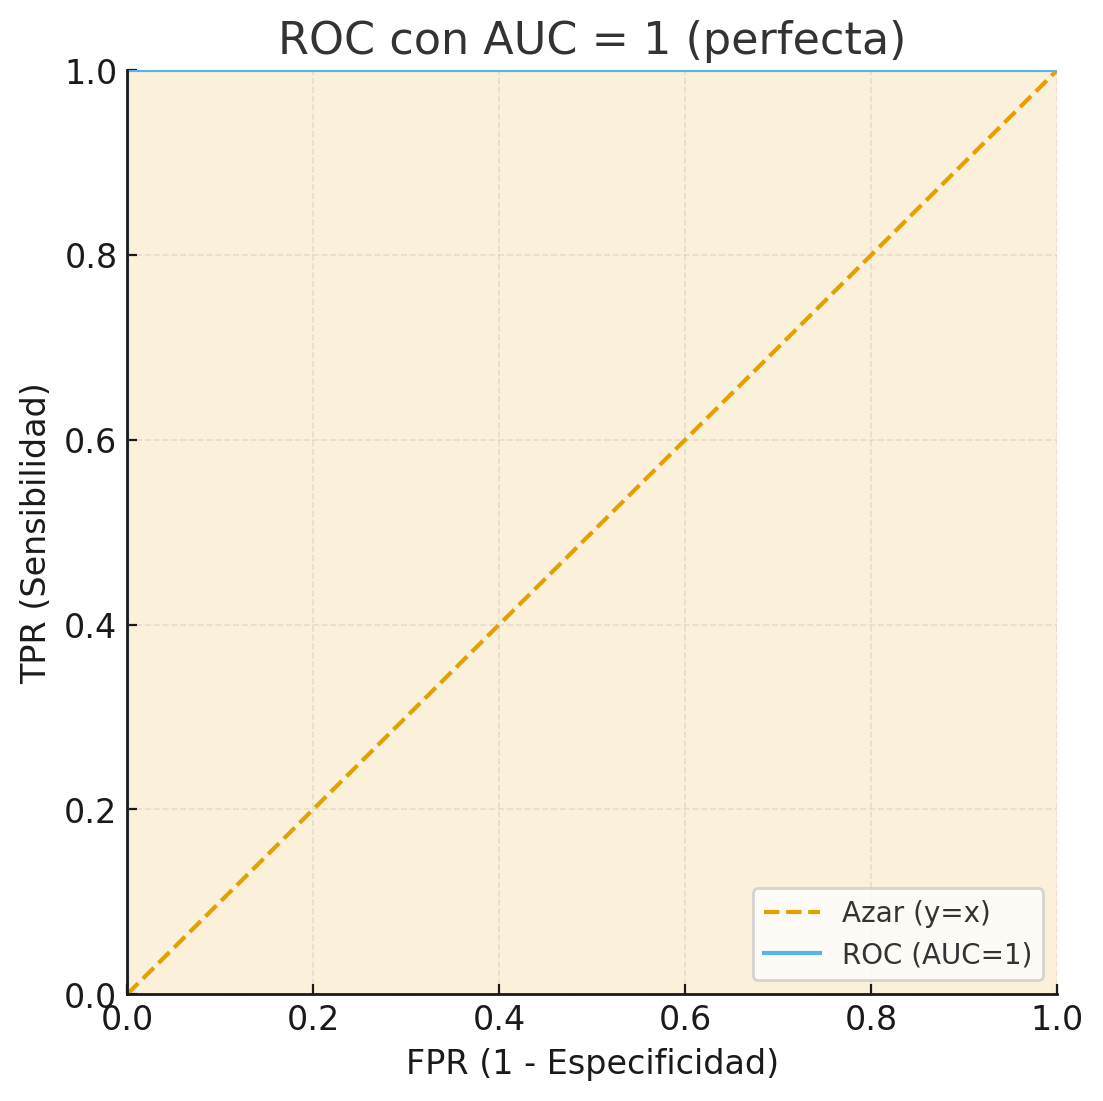
\includegraphics[width=0.45\linewidth]{figs-1/3c.png}
            \end{center}
        \subsection*{Inciso D}
            \begin{center}
                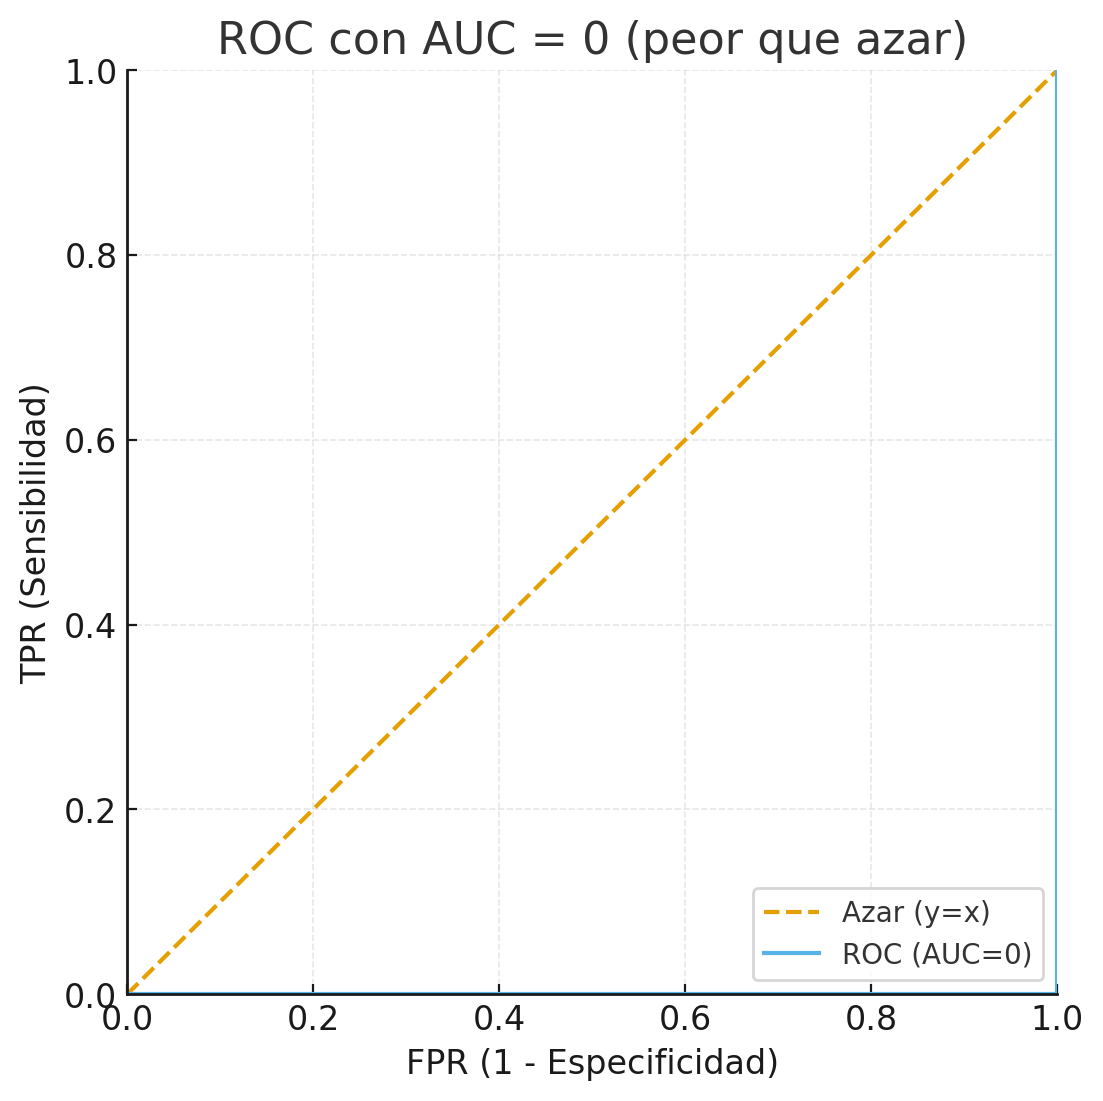
\includegraphics[width=0.45\linewidth]{figs-1/3d.png}
            \end{center}
        \subsection*{Inciso E}
            \begin{center}
                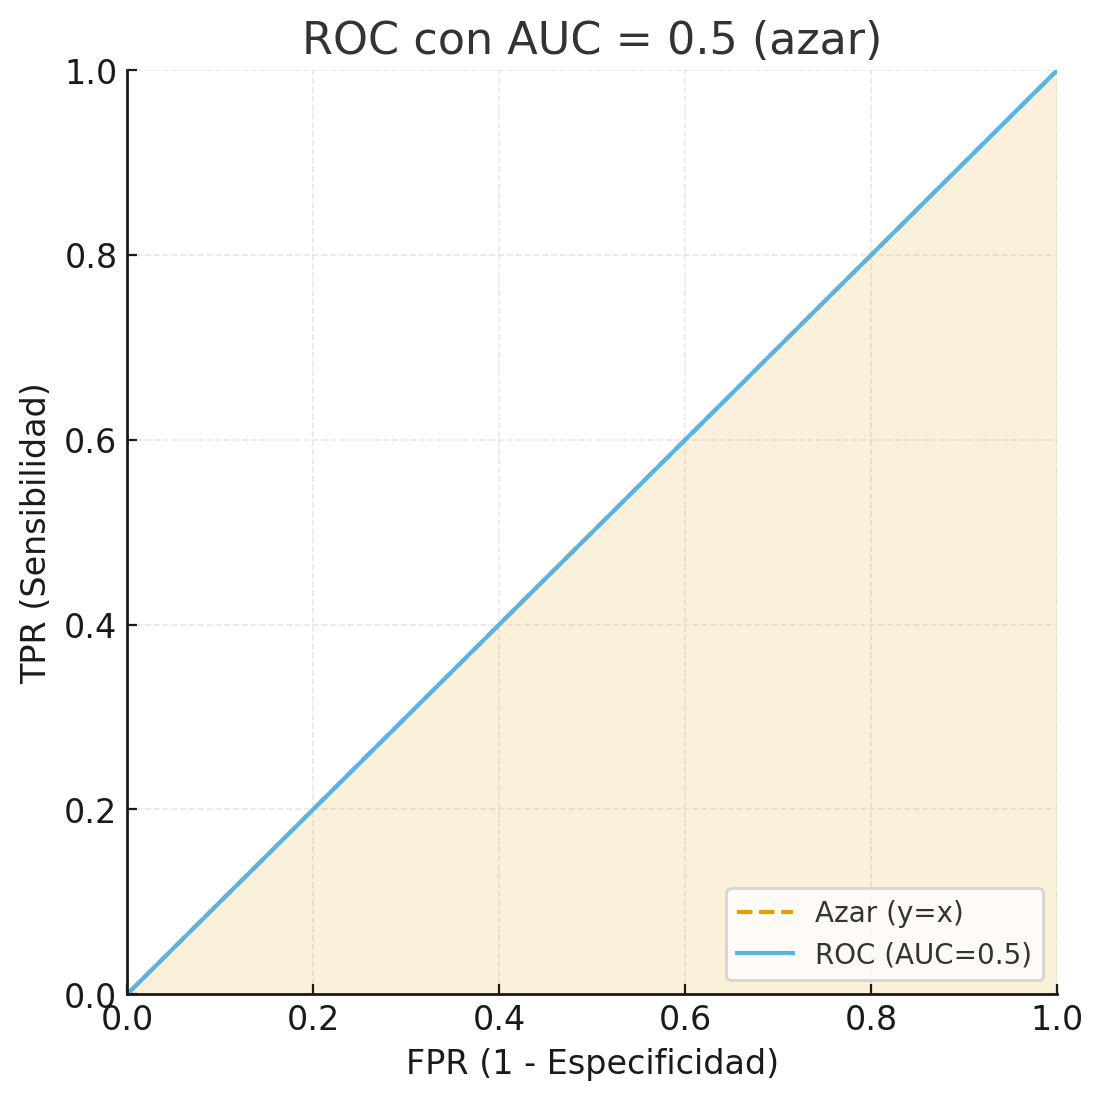
\includegraphics[width=0.45\linewidth]{figs-1/3e.png}
            \end{center}
        \subsection*{Inciso F}
            \begin{center}
                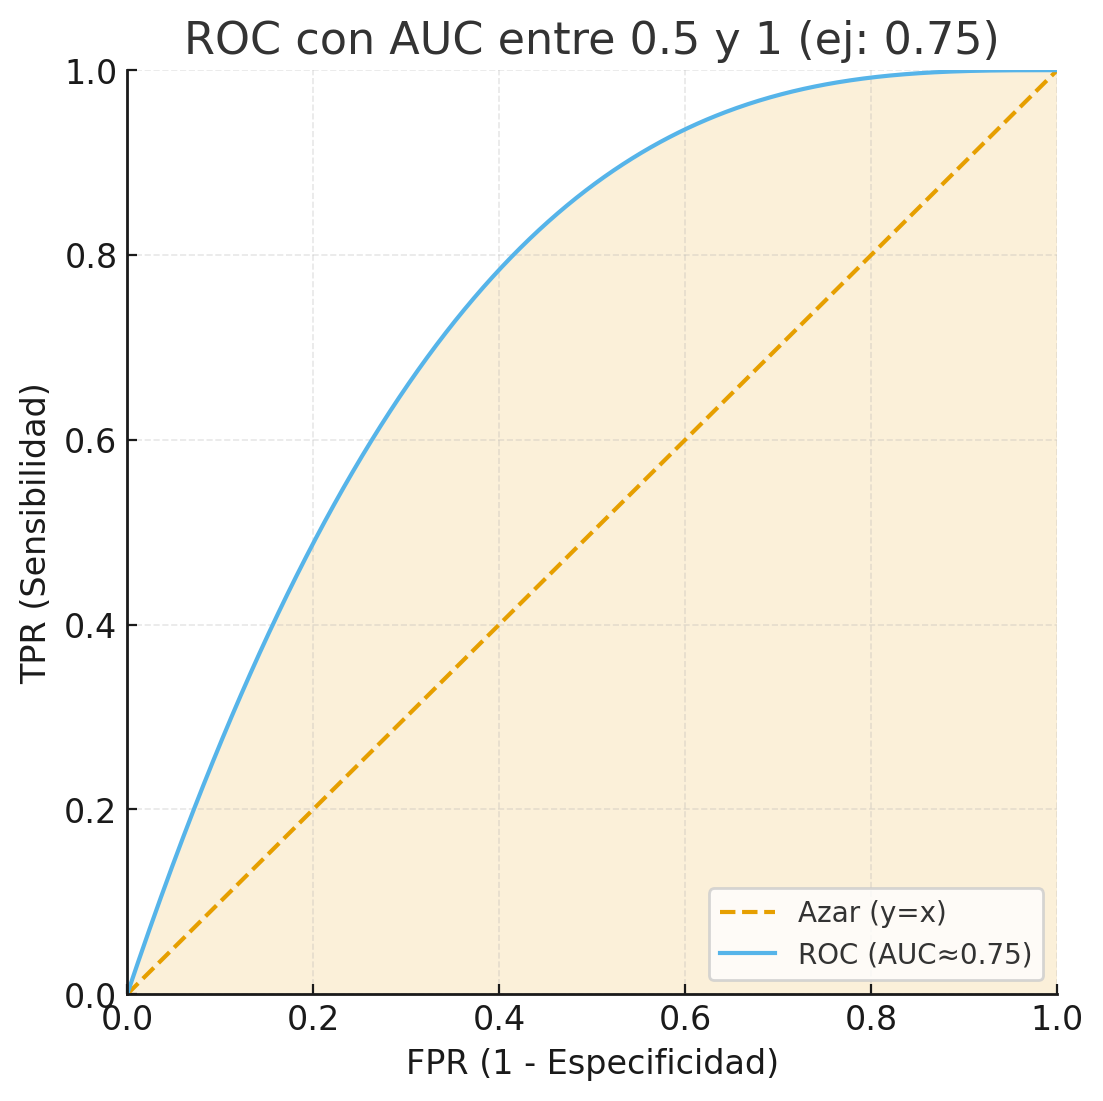
\includegraphics[width=0.45\linewidth]{figs-1/3f.png}
            \end{center}
    \section*{Ejercicio 4}
        \subsection*{Inciso A}
            \textit{Label encoding}, \textit{target encoding}, \textit{embeddings} y \textit{hashing trick}.
        \subsection*{Inciso B}
            Solamente \textit{ordinal encoding}.
        \subsection*{Inciso C}
            Puede quedar la fila completamente inutilizable, llena de \texttt{NA}. Además, no todos los modelos son compatibles con missings. \\
            Para solventar este problema, se puede generar una columna extra para manejar los valores \texttt{NA} en un atributo. Puede llegar a servir un missing a la hora de predecir. Otra posibilidad es quitar el missing y asignar el valor más frecuente de ese atributo.
    \section*{Ejercicio 6}
        \subsection*{Inciso A}
            Si le hacemos una oferta a un no-churner (un falso positivo) va a ser costoso para la empresa, por eso el banco piensa ser más selectivo y enviar pocas ofertas a clientes. Por eso, conviene maximizar precision. Para hacerlo, conviene usar un \(\beta < 1\) porque va cambiar premia los modelos con alta precision aunque tengan menos recall.
        \subsection*{Inciso B}
            \begin{center}
                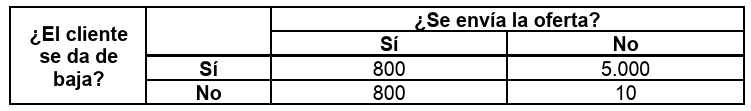
\includegraphics[width=0.45\linewidth]{figs-1/6b.png}
            \end{center}

    
\end{document}
